%!TEX TS-program = xelatex
\documentclass[main]{subfiles}
%这是一个子文件,单独编译时会自动导入main文件的导言区
%这里可以放自定义命令,不会和别人的冲突请放心
%但是不能放newtheorem等高级命令,需要请在群里说
%下面是一些数学命令的简化,可以保留,可以删去,也可以按你的习惯修改
\def\e{\textup{e}}
\def\i{\textup{i}}
\def\T{\textup{T}}
\def\diag{\textup{diag}}
\def\id{\textup{id}}
\newcommand{\toi}[1]{{#1}\to\infty}
\newcommand{\dis}{\displaystyle}
\newcommand{\bv}{\mathrm{BV}}
\newcommand{\ac}{\mathrm{AC}}
\newcommand{\mr}{\mathbb{R}}
\newcommand{\mn}{\mathbb{N}}
\newcommand{\mq}{\mathbb{Q}}
\newcommand{\mz}{\mathbb{Z}}
\newcommand{\rel}{\text{ rel }}
\newcommand{\sgn}{\operatorname{sign}}
\newcommand{\ve}{\varepsilon}
\newcommand{\bs}{\backslash}
\renewcommand{\ll}{\lim\limits}
\renewcommand{\span}{\operatorname{span}}
\renewcommand{\ker}{\operatorname{Ker}}
\renewcommand{\hom}{\operatorname{Hom}}
\renewcommand{\leq}{\leqslant}
\renewcommand{\geq}{\geqslant}
\begin{document}
\renewcommand{\filename}{subfile18}%在这里填你的文件名,避免\label冲突
%这里开始写你的代码
\captionsetup[figure]{name={图},labelsep=period} 
%\title{No. XXX Theorem}\renewcommand\maketitlehookc{\vspace{-18ex}}\date{}
%\maketitle
\section{柯尼斯堡七桥问题}
\subsection{背景介绍}
十八世纪初, 在东普鲁士的柯尼斯堡(今俄罗斯加里宁格勒), 有两条河流经该地, 将其划分为四片陆地, 由7座桥梁连接. 
当地的居民热衷于一个问题: 一个散步者能否设计出一条路线, 使得他走遍七座桥, 且每座桥只走一次? 
\begin{figure}[h]
 
  \centering
      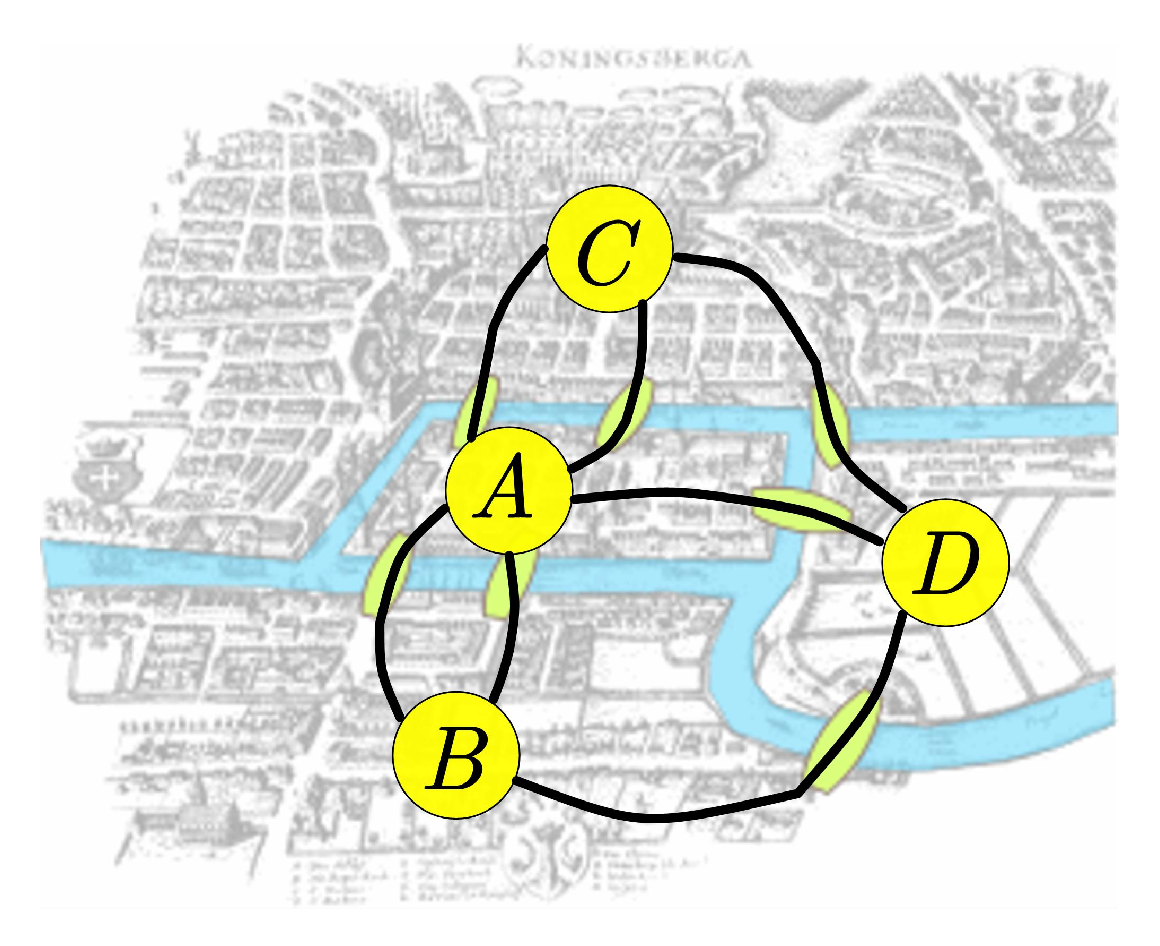
\includegraphics[width=0.45\textwidth]{Konigsberg_bridges.pdf}
      \caption{柯尼斯堡的七座桥}
\end{figure}

这一问题在 Euler 1736年发表的论文《柯尼斯堡的七座桥》中得到解决. 
Euler将问题进行了合适的抽象, 将陆地抽象为\textbf{顶点(vertex)}, 桥抽象为\textbf{边(edge)}, 原始的问题就变成了\textbf{图(graph)}的
一笔画问题: 能否遍历完所有的边而没有重复? 在数学史上, 柯尼斯堡七桥问题的解被认为是图论的第一个定理, 网络理论的第一个
正确的证明, 以及拓扑学(位置几何学)的开端之一.

\subsection{问题的解法}
首先我们定义一个顶点上边的条数为它的\textbf{度数(degree)}, 度数为奇数的我们称其为奇顶点, 度数为偶数的我们称其为偶顶点; 一笔画经过的第一个顶点称起点, 最后一个顶点称终点; 
对于每一个顶点, 一笔画时由另一个顶点画向它的边称进入边, 由它画向另一个顶点的边称离开边. \\
我们可以论证以下能够一笔画的图的性质: 
\begin{enumerate}
  \item 一个图能被一笔画出, 则它一定是连通的(任取两个顶点都存在一条路径将其连接);
  \item 任取一个不是起点和终点的顶点, 由于进入边和离开边成对出现, 其必须是偶顶点;
  \item 由起点出发的一条离开弧没有对应的进入弧, 画向终点的最后一条进入弧没有对应的离开弧; 若起点和终点不同, 则此图必有2个奇顶点; 若起点和终点相同, 则此图没有奇顶点;
\end{enumerate}

对于柯尼斯堡七桥问题, 我们统计它每个顶点的度数: A度数为5, B,C,D度数为3.
则它的奇顶点数有四个, 与前面的性质3矛盾, 故我们断言七桥问题的图不能一笔画. 
\subsection{一笔画定理}
最后,我们介绍一笔画问题的一般判定法.上面给出的一笔画问题的必要条件事实上也是充分条件.具体的证明和更多的背景请阅读\textbf{王敬赓《直观拓扑》}p57
\begin{theorem}[一笔画定理]
  一个图能被一笔画出当且仅当它是连通的, 且奇顶点个数为0或2.
\end{theorem}

\end{document}
